\section{The Data}
\label{sec:data}

In this study, we use the kinematic ages of Kepler field stars, plus stars in
open clusters, to calibrate a new gyrochronology model.
We used the sample of open cluster stars assembled and described in
\citet{curtis2020}, which includes the Pleiades \citep[120 Myr][]{rebull2016},
Praesepe \citep[670 Myr][]{douglas2017, douglas2019},
NGC 6811 \citep[1.0 Gyr][]{curtis2019}, NGC 6819
\citep[2.5 Gyr][]{meibom2015}, and Ruprecht 147 \citep[2.7 Gyr][]{curtis2020}.
We also included the Sun as a data point in our calibration sample with the
following properties: $P_\mathrm{rot, \odot} = 26$ days, Age$_\odot$ = 4.56
Gyr, \gcolor$_\odot$ = 0.82 \citep{citations}.

The field stars in our sample are all in the original \kepler\ field.
This is partly because \kepler\ provides the largest samples of homogeneously
measured rotation periods, and partly because its low Galactic latitude allows
us to marginalize over missing RV measurements and precisely infer vertical
velocity, \vz.
We combined two large rotation period catalogs constructed from original
\kepler\ data: \mct\ and \sant.
These two studies used different techniques to measure rotation periods from
\kepler\ light curves: autocorrelation functions and wavelets respectively.
The \citet{santos2019} study was specifically focused on cooler stars: K and M
dwarfs, and includes a larger number of rotation periods for these stars.
The combined catalogs provided rotation periods for a total of 38,710 stars.

We used the publicly available \kepler-Gaia DR2 crossmatched
catalog\footnote{Available at gaia-kepler.fun} to combine the \mct\ and \sant\
rotation catalogs with the Gaia DR2 catalog of parallaxes, proper motions
and apparent magnitudes.
Reddening and extinction from dust was calculated for each star using the
Bayestar dust map implemented in the {\tt dustmaps} {\it Python} package
\citep{green2018}, and {\tt astropy} \citep{astropy2013, astropy2018}.
We used Gaia DR2 photometric color, $G_{\rm BP} - G_{\rm RP}$, to estimate
effective temperatures for the stars in our sample, using the calibrated
relation in \citet{curtis2020}.

% Unlike isolated main-sequence stars, the rotation periods of binary stars and
% subgiants cannot always be determined by their mass and age (or at least they
% do not always follow the {\it same} gyrochronology relationship as isolated
% dwarfs).
% Photometric binaries and subgiants were therefore removed from the sample by
% applying cuts to the color-magnitude diagram (CMD), shown in figure
% \ref{fig:CMD}.
% A 6th-order polynomial was fit to the main sequence and raised by 0.27 dex to
% approximate the division between single stars and photometric binaries (shown
% as the curved dashed line in figure \ref{fig:CMD}).
% All stars above this line were removed from the sample.
% Potential subgiants were also removed by eliminating stars brighter than 4th
% absolute magnitude in Gaia G-band.
% This cut also removed a number of main sequence F stars from our sample,
% however these hot stars are not the focus of our gyrochronology study since
% their small convective zones inhibit the generation of a strong magnetic
% field.
% The removal of photometric binaries and evolved/hot stars reduced the total
% sample of around 38,000 stars by around 4,000.

3705 stars in our sample had RV measurements available in Gaia DR2, with a
median uncertainty of 1.88 \kms.
Gaia DR2 included RVs for stars with Gaia apparent magnitudes between 4
and 13, and 3550 K $\lesssim$ \teff\ $\lesssim$ 6900 K \citep{brown2018}.
We also crossmatched the \mct\ sample with the 5th LAMOST data release
\citep{cui2012, xiang2019}, adding a further 10623 RV measurements to the
sample, and expanding the total number of stars with measured RVs to 14,328.
The median uncertainty of the LAMOST RV measurements was 4.71 \kms\ and,
given that the Gaia RVs were more precise, on average, than the LAMOST
RVs, we adopted the Gaia value in cases where both were available.
We note that the third Gaia data release will contain a large number of new
RV measurements for the stars in our sample.

We removed stars with a Gaia parallax signal-to-noise ratio of less than 10,
stars with negative parallaxes, and stars with a Gaia astrometric excess noise
value greater than 5.
After these cuts, 35,328 stars remained in our sample, of which 11,050 had RV
measurements from either Gaia or LAMOST.
We calculated 3D velocities for all stars with measured RVs using {\tt
astropy}, and {\it inferred} 3D velocities for the remaining 24,278 stars
using the method described in section \ref{sec:velocities}.
\racomment{check these numbers are consistent.}

\subsection{Kinematic ages}
\label{sec:kinematic_ages}

After calculating the vertical velocities of these stars using the method
described below, we then calculated a kinematic age for each star using the
method described in \citet{lu2021}.
A kinematic age can be calculated from the velocity dispersion, \ie\ standard
deviation of velocities, of a group of stars.
Velocity dispersion can then be converted into an age using an AVR
\citep[\eg][]{holmberg2009, yu2018}.
In \citet{lu2021} the kinematic ages of Kepler stars were calculated by
binning them in rotation period, effective temperature, absolute Gaia
magnitude and Rossby number-space.
The kinematic age of each star was estimated by calculating the velocity
dispersions of stars with similar parameters, and using an AVR to calculate a
corresponding age.
The bin size was optimized using a number of Kepler stars with asteroseismic
ages.
This kinematic age-dating method produced ages that were consistent with
independent measurements of stellar age, for stars with available ages (stars
in open clusters and asteroseismic stars, primarily).
The uncertainties on these kinematic ages were estimated to be around 1-2 Gyr.
Further details of this kinematic dating method are provided in that work.

% Kinematic ages represent the {\it average age} of a group of stars and are
% most informative when stars are grouped by age.
% If a group of stars have similar ages, their kinematic age will be close
% the age of each individual.
% On the other hand, the kinematic age of a group with large age variance will
% not provide much information about the ages of individual stars.
% Velocity distributions themselves do not reveal whether a group of stars have
% similar or different ages, since either case the velocities are
% Gaussian-distributed.
% Fortunately however, we can group \kepler\ stars by age using the implicit
% assumption that underpins gyrochronology: that stars with the same rotation
% period and color are the same age.
% % We discuss the implications of this assumption and cases where it doesn't
% % apply in the Discussion of this paper (section \ref{sec:discussion}).

% We used the \citet{yu2018} AVR to convert velocity dispersion to age.
% This relation was calibrated using the ages and velocities of red clump stars.
% They divided their sample into metal rich and poor subsets, and calibrated
% separate AVRs for each, plus a global AVR.
% Their AVR is a power law:
% \begin{equation}
%     \sigma_{vz} = \alpha t ^\beta,
% \end{equation}
% where $\alpha$ and $\beta$ take values (6.38, 0.578) for metal rich stars
% (3.89, 1.01) for metal poor stars, and (5.47, 0.765) for all stars.

% We used 1.5$\times$ the Median Absolute Deviation (MAD) of velocities, which
% is a robust approximation to the standard deviation and is less sensitive to
% outliers.
% Velocity outliers could be binary stars or could be generated by
% underestimated parallax or proper motion uncertainties.

Figure \ref{fig:kin_and_clusters} displays the data we used to calibrate our
gyrochronology model in \prot-\teff\ space.
Kepler field stars are shown as small points, and cluster stars are larger
points with black outlines.
Points are colored by either their kinematic ages or cluster ages.
The left- and right-hand panels have a linear and logarithmic y-axis,
respectively.

\begin{figure}
\caption{
    The calibration data.
Kepler field stars are shown as small points, and cluster stars are larger
points with black outlines.
Points are colored by either their kinematic ages or cluster ages.
The left- and right-hand panels have a linear and logarithmic y-axis,
respectively.
}
  \centering 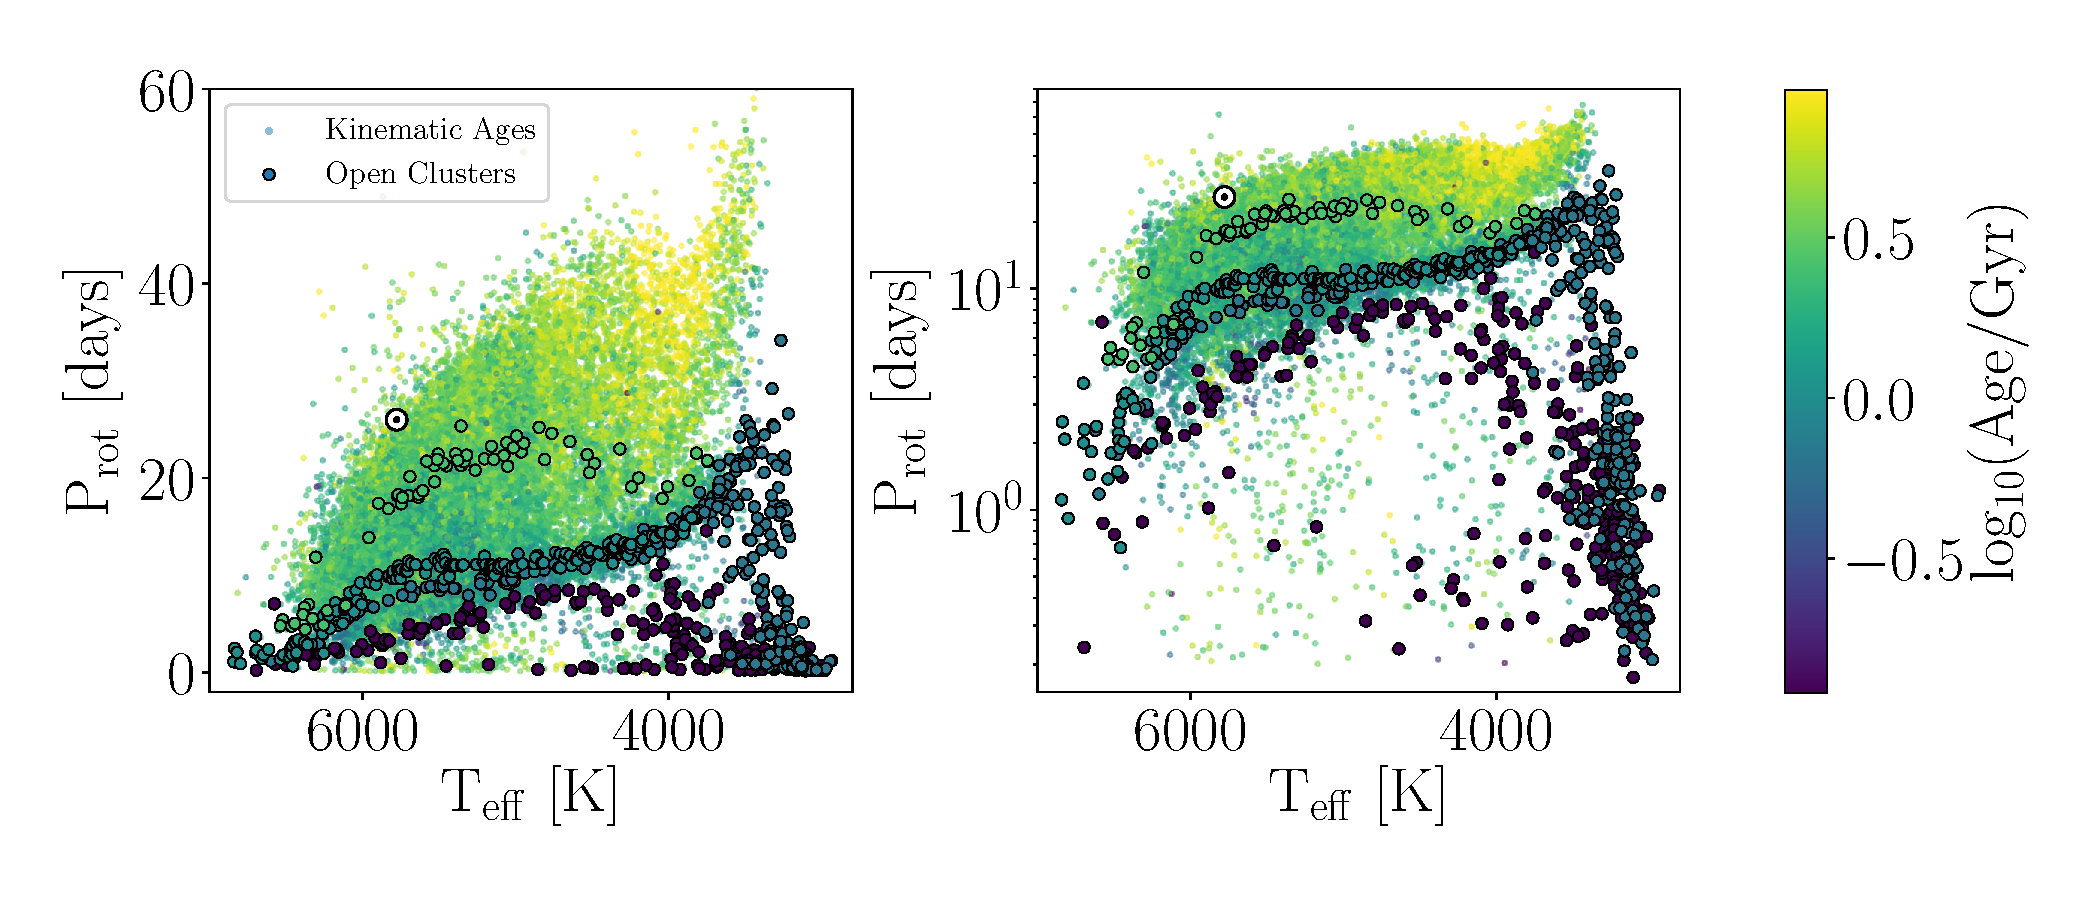
\includegraphics[width=1\textwidth]{kin_and_clusters_log_lin}
\end{figure}
